documentclass[border=10pt]{standalone}
\usepackage{tikz}

\begin{document}

\begin{figure}[h]
\begin{center}
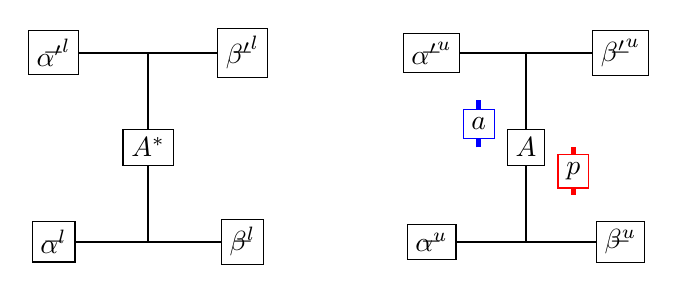
\begin{tikzpicture}[scale=1.2]
\begin{scope}[local bounding box=(a)]
\draw[black, thick] (-1,-1) -- (1,-1);
\node [draw=black, inner sep=3pt, fill=white] at (-1,-1) (alpha){$\alpha^{l}$};
\node [draw=black, inner sep=3pt, fill=white] at (1,-1) (beta){$\beta^{l}$};
\draw[black, thick] (-1,1) -- (1,1);
\node [draw=black, inner sep=3pt, fill=white] at (-1,1) (alpha'){${\alpha'}^{l}$};
\node [draw=black, inner sep=3pt, fill=white] at (1,1) (beta'){${\beta'}^{l}$};
\draw[black, thick] (0,-1) -- (0,1);
\node [draw=black, inner sep=3pt, fill=white] at (0,0) (A) {$A^{*}$};

\node[anchor=center] at (alpha.center) {$-$};
\node[anchor=center] at (alpha'.center) {$-$};
\node[anchor=center] at (beta.center) {$-$};
\node[anchor=center] at (beta'.center) {$-$};

\end{scope}

\begin{scope}[local bounding box=(b), xshift=4cm]
\draw[black, thick] (-1,-1) -- (1,-1);
\node [draw=black, inner sep=3pt, fill=white] at (-1,-1) (alpha){$\alpha^{u}$};
\node [draw=black, inner sep=3pt, fill=white] at (1,-1) (beta){$\beta^{u}$};
\draw[black, thick] (-1,1) -- (1,1);
\node [draw=black, inner sep=3pt, fill=white] at (-1,1) (alpha'){${\alpha'}^{u}$};
\node [draw=black, inner sep=3pt, fill=white] at (1,1) (beta'){${\beta'}^{u}$};
\draw[black, thick] (0,-1) -- (0,1);
\node [draw=black, inner sep=3pt, fill=white] at (0,0) (A) {$A$};

\draw[blue, line width=0.6mm] (-0.5,0)--(-0.5,0.5); %\node [draw=blue, inner sep=0pt, minimum size=0.5cm] at (-0.5,0) {};
\node[draw=blue, inner sep=3pt, fill=white] at (-0.5,0.25) (a) {$a$};
\node[anchor=center] at (alpha.center) {$-$};
\node[anchor=center] at (alpha'.center) {$-$};
\node[anchor=center] at (beta.center) {$-$};
\node[anchor=center] at (beta'.center) {$-$};

\draw[red, line width=0.6mm] (0.5,0)--(0.5,-0.5); %\node [draw=red, inner sep=0pt, minimum size=0.5cm] at (0.5,0) {};
\node[draw=red, inner sep=3pt, fill=white] at (0.5,-0.25) (p) {$p$};
\end{scope}
\end{tikzpicture}
\caption{Transfer matrices corresponding to (a) weak injectivity in Eq.~(\ref{weak transfer matrix}) and (b) strong injectivity in Eq.~(\ref{strong transfer matrix}). }
\end{center}
\end{figure}

\end{document}